\documentclass[12pt]{article}

\usepackage[margin = .8in]{geometry}
\usepackage{amsmath}
\usepackage{graphicx}
\usepackage{multicol, enumerate, tabularx}
\usepackage{booktabs}
\usepackage{array}
\usepackage{adjustbox}

\usepackage{fancyhdr}
\pagestyle{fancy}

\lhead{Math F113X: Math and Society}
\rhead{Date: \hspace{1in}}

\usepackage{tikz}
\usetikzlibrary{calc,trees,positioning,arrows,fit,shapes,through, backgrounds}
\usetikzlibrary{patterns}

\usetikzlibrary{decorations.markings}
\usetikzlibrary{arrows}

\usepackage{pgfplots}

\usepackage{longtable}
\usepackage{tabularx}

\newcommand{\ds}{\displaystyle}
\newcommand{\ans}[1][1in]{\rule{#1}{.5pt}}

\newcommand{\points}[1]{(#1 points.)}		% Trying to be lazy.

\usepackage{array}
\newcolumntype{L}[1]{>{\raggedright\let\newline\\\arraybackslash\hspace{0pt}}m{#1}}
\newcolumntype{C}[1]{>{\centering\let\newline\\\arraybackslash\hspace{0pt}}m{#1}}
\newcolumntype{R}[1]{>{\raggedleft\let\newline\\\arraybackslash\hspace{0pt}}m{#1}}
\newcommand{\red}[1]{\textcolor{red}{#1}}

\newcommand{\be}{\begin{enumerate}}
\newcommand{\ee}{\end{enumerate}}

%\topmargin -1in
%\textheight 9.5in
%\oddsidemargin -0.3in
%\evensidemargin \oddsidemargin
%\pagestyle{empty}
%%\marginparwidth 0.5in
%\textwidth 7in
%\parindent 0in

%--------------------------------------------------------------------------------------------------------------------------------------------------------------------------
%						Document
%--------------------------------------------------------------------------------------------------------------------------------------------------------------------------


\begin{document}
%\pagestyle{fancy}
\begin{center}
{\Large  Worksheet 14 (Graph Theory 6): Hamiltonian Circuits }
\end{center}



%\noindent \textbf{Group Names:} \hrulefill \\
%-------------------------------------------------------------------------------------------------------------
%						Assignment
%-----------------------------------------------------------------------------------------------------
\begin{enumerate}


\item Draw two different Hamiltonian circuit in the graph below. Below each graph, list the vertices of your circuit in order.\\


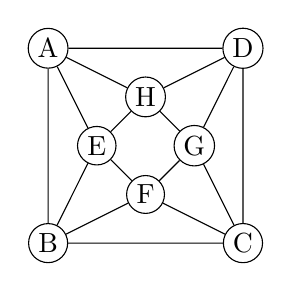
\begin{tikzpicture}[scale=1.75]
\tikzstyle{every node}=[circle, draw, fill=white,
                        inner sep=1.5pt]
\node (1) at (-0.707, 0.707){A};
\node (2) at (-0.707, -0.707){B};
\node (3) at (0.707, -0.707){C};
\node (4) at (0.707, 0.707){D};
\node (5) at (-0.354, 0.){E};
\node (6) at (0., -0.354){F};
\node (7) at (0.354, 0.){G};
\node (8) at (0., 0.354){H};
\foreach \i/\j in {1/2,1/4,1/5,1/8,2/3,2/5,2/6,3/4,3/6,3/7,4/7,4/8,5/6,5/8,6/7,7/8}{\draw (\i) -- (\j);}
\end{tikzpicture}
\hfill
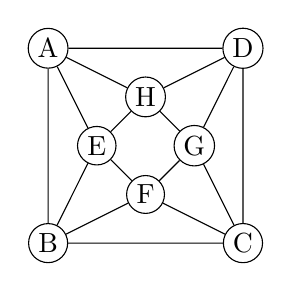
\begin{tikzpicture}[scale=1.75]
\tikzstyle{every node}=[circle, draw, fill=white,
                        inner sep=1.5pt]
\node (1) at (-0.707, 0.707){A};
\node (2) at (-0.707, -0.707){B};
\node (3) at (0.707, -0.707){C};
\node (4) at (0.707, 0.707){D};
\node (5) at (-0.354, 0.){E};
\node (6) at (0., -0.354){F};
\node (7) at (0.354, 0.){G};
\node (8) at (0., 0.354){H};
\foreach \i/\j in {1/2,1/4,1/5,1/8,2/3,2/5,2/6,3/4,3/6,3/7,4/7,4/8,5/6,5/8,6/7,7/8}{\draw (\i) -- (\j);}
\end{tikzpicture}

\vfill
\item  Answer questions about the graph sketched below.\\

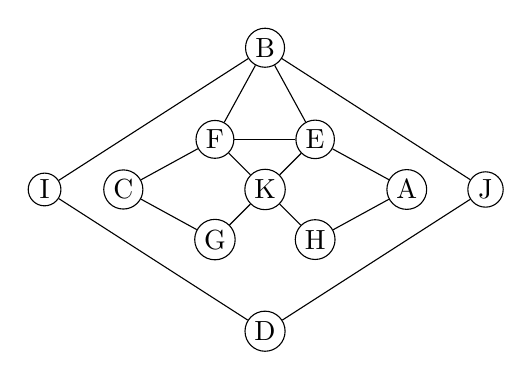
\begin{tikzpicture}[baseline=(current bounding box.center),scale = 0.9]
\tikzstyle{every node} = [draw, circle, inner sep = 1.5 pt];
\node (A) at (0:2) {A};
\node (B) at (90:2) {B};
\node (C) at (180:2) {C};
\node (D) at (270:2) {D};
\node (O) at (0,0){K};
\node (E) at (45:1) {E};
\node (F) at (45+90:1){F};
\node (G) at (45+180:1){G};
\node (H) at (45+270:1){H};
\node[left of = C] (I) {I};
\node [right of = A] (J) {J};
\draw (B) -- (I) -- (D) -- (J)--(B);
\draw (A) -- (E) -- (B) -- (F) -- (C);
\draw (E) -- (O) -- (G) (F) --(O) --(H);
\draw (C) -- (G) (H) --(A);
\draw (E) -- (F) ;
\end{tikzpicture}

	\be
	\item Draw a Hamiltonian path starting at vertex I. List the vertices of your circuit in order.
	\vfill
	\item Draw a Hamiltonian path starting at vertex B or explain why this is not possible.
	\vfill
	\item  Find a Hamiltonian \emph{circuit} or explain why this is not possible.
	\vfill
	\ee
\newpage






\item List \emph{every} possible Hamiltonian circuit in the graph below. Give a numerical justification that you have all of them.

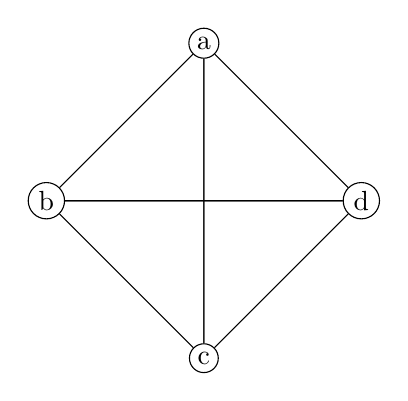
\begin{tikzpicture}[vtx/.style={draw, circle, inner sep =1.5 pt}, lbl/.style =  {inner sep =1.5 pt, fill = white}]
\foreach \i/\lbl in {0/a, 1/b, 2/c, 3/d}{
  \node[vtx] (\i) at (360*\i/4+90:2){\lbl};
}
\foreach \i in {0,1,2,3}{
  \draw let \n1 = {int(mod(\i+1,4))}, \n2 = {int(mod(\i+2,4))}, \n3 = {int(mod(\i+2,4))}
  	in (\i) -- (\n1) (\i) -- (\n2) (\i) -- (\n3);
}

\end{tikzpicture}
\vfill
\item The following graph has two different Hamiltonian circuits. Highlight one on each copy of the graph and compute the total weight of the circuit.  

\bigskip

\begin{tabularx}{\linewidth}{X X}
\fbox{Circuit 1} & \fbox{Circuit 2}\\
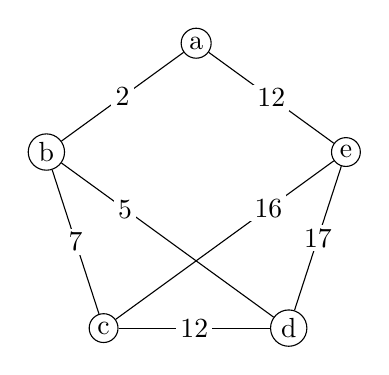
\begin{tikzpicture}[vtx/.style={draw, circle, inner sep =1.5 pt}, lbl/.style =  {inner sep =1.5 pt, fill = white}]
\foreach \i/\lbl in {0/a, 1/b, 2/c, 3/d, 4/e}{
  \node[vtx] (\i) at (360*\i/5+90:2){\lbl};
}
\foreach \i in {0,1,2,3,4}{
  \draw let \n1 = {int(mod(\i+1, 5))}, \n2 = {int(3*\i+2*\n1)}
    in (\i) -- node[lbl] {\n2} (\n1);
}
\draw (1) -- node[pos=.3, lbl] {5}  (3);
\draw (2) -- node[pos=.7, lbl] {16} (4);

\end{tikzpicture}
&
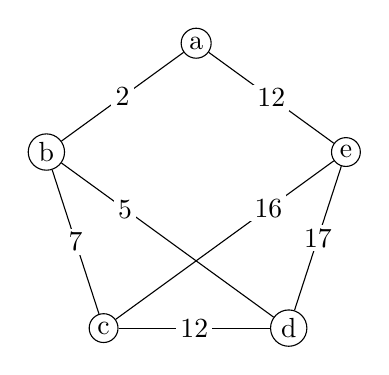
\begin{tikzpicture}[vtx/.style={draw, circle, inner sep =1.5 pt}, lbl/.style =  {inner sep =1.5 pt, fill = white}]
\foreach \i/\lbl in {0/a, 1/b, 2/c, 3/d, 4/e}{
  \node[vtx] (\i) at (360*\i/5+90:2){\lbl};
}
\foreach \i in {0,1,2,3,4}{
  \draw let \n1 = {int(mod(\i+1, 5))}, \n2 = {int(3*\i+2*\n1)}
    in (\i) -- node[lbl] {\n2} (\n1);
}
\draw (1) -- node[pos=.3, lbl] {5}  (3);
\draw (2) -- node[pos=.7, lbl] {16} (4);

\end{tikzpicture}\\[16 pt]
Weight: \ans & Weight: \ans
\end{tabularx}

\vspace{1cm}

Which Hamiltonian circuit has the smallest weight? \ans

\item Recall that Kruskal's Algorithm found a minimum weight spanning tree by selecting the cheapest edges that don't form a circuit. Do you think such an algorithm can be modified to find a minimum weight Hamiltonian circuit? What modifications would be needed? What might be some challenges?
\vfill


\end{enumerate}
\end{document}

%-------------------------------------------------------------------------------------------------------------------------------------------------------------------------------------------------------------------

%%% Local Variables:
%%% mode: latex
%%% TeX-master: t
%%% End:
